7. \begin{figure}[ht!]
\center{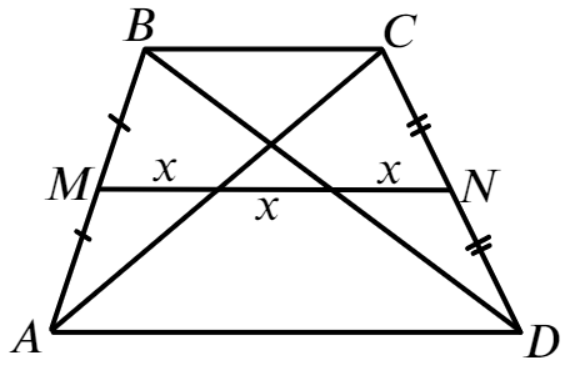
\includegraphics[scale=0.35]{g8-7.png}}
\end{figure}\\
Так как отрезок $MN$ является средней линией трапеции, он параллелен основаниям и проходит через середины $AB$ и $CD,$ а поэтому также содержит средние линии треугольников $ABC$ и $ABD.$ Тогда $x=\cfrac{1}{2}BD$ и $2x=\cfrac{1}{2}AD,$ откуда $BC=2x,\ AD=4x$ и $\cfrac{BC}{AD}=\cfrac{2x}{4x}=\cfrac{1}{2}.$\\
